\documentclass{beamer}

\usepackage{amssymb,amsmath}
\usepackage{graphicx}
\usepackage{url}
\usepackage{color}
\usepackage{pagenote}[continuous,page]
\usepackage{relsize}		% For \smaller
\usepackage{url}			% For \url
\usepackage{epstopdf}	% Included EPS files automatically converted to PDF to include with pdflatex

%For MindMaps
% \usepackage{tikz}%
% \usetikzlibrary{mindmap,trees,arrows}%

%%% Color Definitions %%%%%%%%%%%%%%%%%%%%%%%%%%%%%%%%%%%%%%%%%%%%%%%%%%%%%%%%%
%\definecolor{bordercol}{RGB}{40,40,40}
%\definecolor{headercol1}{RGB}{186,215,230}
%\definecolor{headercol2}{RGB}{80,80,80}
%\definecolor{headerfontcol}{RGB}{0,0,0}
%\definecolor{boxcolor}{RGB}{186,215,230}

%%% Save space in lists. Use this after the opening of the list %%%%%%%%%%%%%%%%
%\newcommand{\compresslist}{
%	\setlength{\itemsep}{1pt}
%	\setlength{\parskip}{0pt}
%	\setlength{\parsep}{0pt}
%}

%\setbeameroption{show notes on top}

% You should run 'pdflatex' TWICE, because of TOC issues.

% Rename this file.  A common temptation for first-time slide makers
% is to name it something like ``my_talk.tex'' or
% ``john_doe_talk.tex'' or even ``discrete_math_seminar_talk.tex''.
% You really won't like any of these titles the second time you give a
% talk.  Try naming your tex file something more descriptive, like
% ``riemann_hypothesis_short_proof_talk.tex''.  Even better (in case
% you recycle 99% of a talk, but still want to change a little, and
% retain copies of each), how about
% ``riemann_hypothesis_short_proof_MIT-Colloquium.2000-01-01.tex''?

\mode<presentation>
{
  \usetheme{CambridgeUS}		% bem bacana - menu superior
  \usecolortheme{default}		% branco, azul clarinho
  \useoutertheme{default}
  \useinnertheme{circles}
  \setbeamercovered{invisible}
}

\beamertemplatenavigationsymbolsempty

%% Better looking blocks
\setbeamercolor{block title alerted}{use=structure,fg=black,bg=red!80!black}
\setbeamercolor{block body alerted}{use=structure,fg=black,bg=white!90!black}

\setbeamercolor{block title}{use=structure,fg=black,bg=blue!60!white}
\setbeamercolor{block body}{use=structure,fg=black,bg=white!90!black}

\usepackage[english]{babel}
\usepackage[latin1]{inputenc}
\usepackage{subfigure}

\usepackage{times}
\usepackage[T1]{fontenc}

%% makes the ppagenote command for figure references at the end.
\makepagenote
\renewcommand{\notenumintext}[1]{}
\newcommand{\ppagenote}[1]{\pagenote[Page \insertframenumber]{#1}}


\title[GB13604]{GB13604 - Maths for Computer Science}
\subtitle[]{Lecture 1 -- Intro, and Intro to Proofs}
\author[Claus Aranha]{Claus Aranha\\{\footnotesize caranha@cs.tsukuba.ac.jp}}
\institute[COINS]{College of Information Science}
\date[2018-10-03]{2018-10-03\\{\tiny Last updated \today}}

\begin{document}

\section{Introduction}
\subsection{Outline}

\begin{frame}
  \maketitle
\end{frame}

\begin{frame}
  \frametitle{What is this course about?}

  In this course, we study (\structure{or review?}) mathematic
  subjects that are \structure{useful for computer scientists}.

  \vfill
  
  \begin{itemize}
  \item Big topic: Discrete Mathematics
  \item Sub topics:
    \begin{itemize}
    \item Proofs
    \item Sets
    \item Integers
    \item Combinations
    \item Probability
    \end{itemize}
  \end{itemize}

  
  \bigskip

  Also, this course \structure{secondary goal} is to improve your
  \structure{technical English} by usage.
\end{frame}


\begin{frame}
  \frametitle{Course Materials}

  
  This course is based on \structure{Mathematics for Computer Science,
    Spring 2015}, by Albert Meyer and Adam Chlipala, Massachusetts
  Institute of Technology (MIT), OpenCourseWare (OCW)

  \bigskip

  The original MIT materials and all the materials prepared in my
  version of the course are licensed as Creative Commons BY-NC-SA.
  
  \bigskip
  
  \begin{center}
    
\includegraphics[width=0.2\textwidth]{../img/by-nc-sa}
  \end{center}

  \bigskip

  You can find a link to the original course, and the textbook
  download, on MANABA. \alert{Please read the material!}
\end{frame}

\begin{frame}
  \frametitle{Course Structure}

  \begin{itemize}
  \item Overview of the Week's topics;
  \item Presenting the Weekly exercise;
  \item Discussion of the Weekly exercise;
  \end{itemize}

  \bigskip
  \begin{block}{End time}
    If you have finished the exercise and have no more questions, ask
    and you may leave the class early.
  \end{block}
\end{frame}

\begin{frame}
  \frametitle{Course Topics}
  \begin{itemize}
  \item Part I: Proofs
    \begin{itemize}
    \item Class 1: Introduction to Proofs
    \item Class 2: Sets and Induction
    \end{itemize}
  \item Part II: Structures
    \begin{itemize}
    \item Class 1: Number Theory
    \item Class 2: Directed Graphs and Partial Orders
    \item Class 3: Simple and Planar Graphs
    \end{itemize}
  \item Part III: Counting
    \begin{itemize}
    \item Class 1: Sums and Assymptotics
    \item Class 2: Cardinality Rules and Generating Functions
    \end{itemize}
  \item Part IV: Probability
    \begin{itemize}
    \item Class 1: Events, Probability Spaces, Conditionals
    \item Class 2: Random Variables, Deviation from Mean, Random Walk
    \item Class 3: Advanced Topics and Review
    \end{itemize}
  \end{itemize}
\end{frame}

\begin{frame}
  \frametitle{Course Evaluation}
  \begin{itemize}
  \item 50\% Weekly Exercises
    \begin{itemize}
    \item One to three questions will be posed in class;
    \item Students may discuss the answers in class, but the report must be individual;
    \item Submission must be a PDF on MANABA;
    \end{itemize}

    \bigskip
    
  \item 50\% Final Exam
  \end{itemize}

  \vfill

  \begin{block}{Extra Credit}
    I often give extra credit to students who participate in class
    with questions, interesting comments, good suggestions, etc.
  \end{block}
\end{frame}

\begin{frame}
  \frametitle{About the Course Language}

  One of the goals of this lecture is to raise your level of technical
  English. However, this is not an English Class.

  \bigskip
  
  I expect the students to submit their exercises and exam answers in
  English. It does not need to be perfect, but I expect you to make a
  good effort.

  \bigskip

  I recommend that you watch the videos in the MIT OCW website. All
  videos include subtitles.

  \begin{block}{If you are having difficulties}
    Please contact me by MANABA message or by e-mail at any time!
  \end{block}
  
\end{frame}


\begin{frame}
  \frametitle{About the Lecturer}
  \begin{columns}
    \column{0.4\textwidth}
    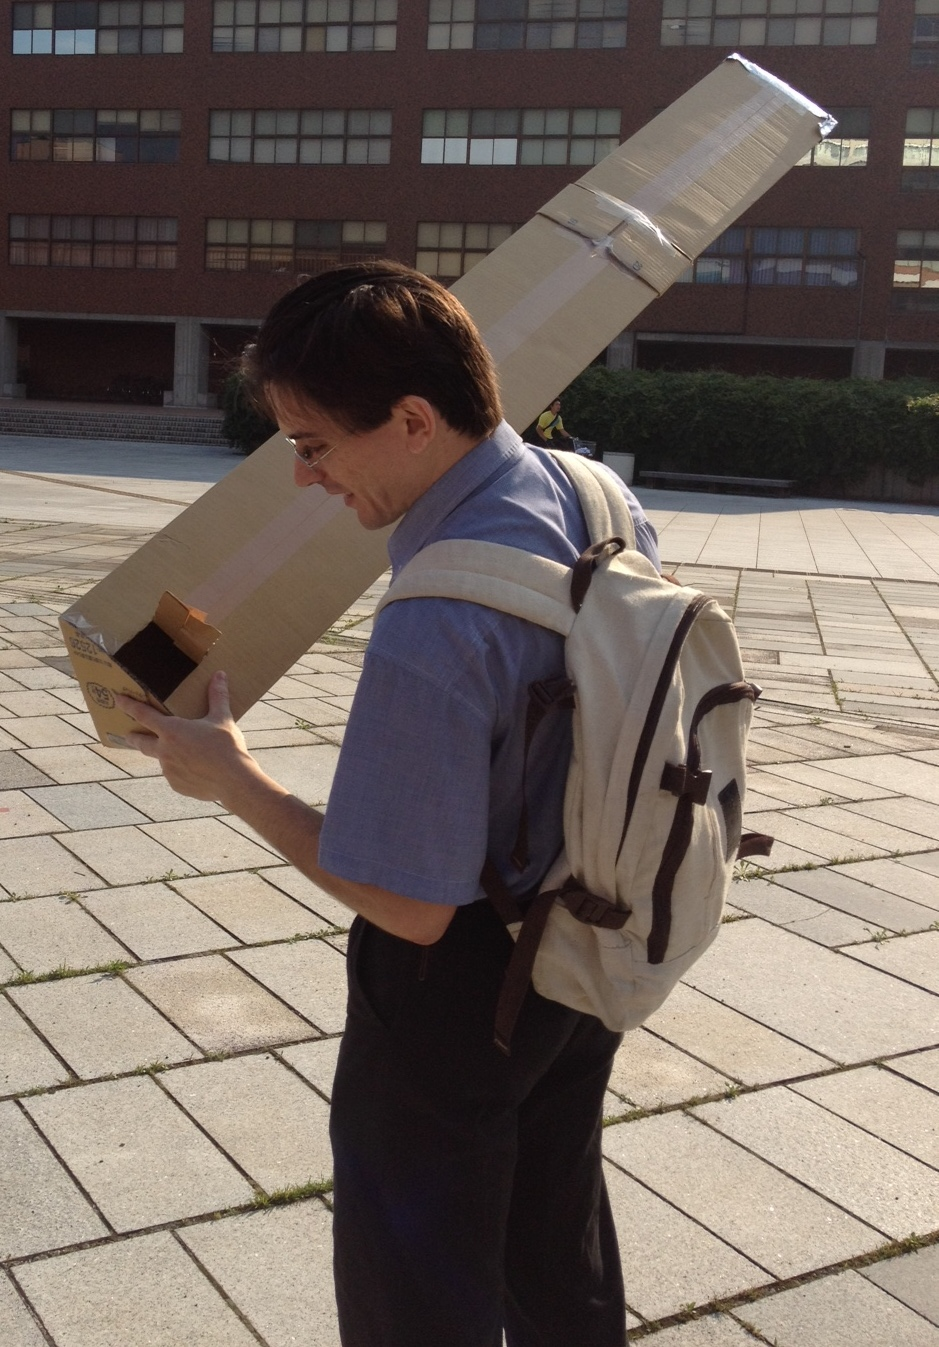
\includegraphics[width=1\textwidth]{../img/pinhole}
    \column{0.6\textwidth}
           {\small
             \begin{itemize}
             \item \structure{Name:} Claus Aranha;
               \medskip
               
             \item \structure{Country:} Brazil;
               \medskip
               
             \item \structure{Research:} Evolutionary Computation,
               Artificial Life, (some) Deep Learning
               \medskip

             \item \structure{Hobby:} PICO-8, Twitter
               \medskip

             \item \structure{Webpage:}
               \url{http://conclave.cs.tsukuba.ac.jp}
             \end{itemize}
           }
  \end{columns}
\end{frame}

\section{1.1 -- Intro to Proofs}

\begin{frame}
  \begin{center}
    Mathematics for Computer Sciences\\
    Part I -- Proofs
  \end{center}
\end{frame}

\subsection{What is a Proof?}

\begin{frame}
  \frametitle{What is a proof?}

  \begin{center}
    \includegraphics[width=0.4\textwidth]{../img/pythagorean_theorem}
  \end{center}
  \begin{itemize}
  \item Proofs are used to show \structure{how you know} something
  \item Proofs are not obvious (more than 100 proofs for pythagoras)
  \end{itemize}
\end{frame}

\begin{frame}[fragile]
  \frametitle{Why are proofs important for Computer Sciences?}

  The techniques and ides of proofs can be used for \alert{debugging}.
  
  \begin{block}{This program outputs the type of triangle}
\begin{verbatim}
int triangle_type(int a, int b, int c)
  if (a == b)
    if (b == c) 
      return "all sides are equal";
    else
      return "two sides are equal";
  else if (b == c) 
    return "two sides are equal";
  else
    return "all sides are different"; 
\end{verbatim}
  \end{block}

  \begin{itemize}
  \item Is this program correct or incorrect?
  \item How can you show it with \structure{confidence}?
  \end{itemize}
\end{frame}

\begin{frame}
  \frametitle{What is a Proof?}

  \begin{itemize}
  \item \structure{A proposition} is a statement that can be
    \structure{True} or \alert{False}.
    \begin{itemize}
    \item This room has 40 chairs.
    \item Every intelligent being feels pain.
    \item Please say your name.
    \item $513 \times 435 = 223165$
    \item Every even integer greater than 2 is the sum of two primes.
    \item It is raining now.
    \end{itemize}

    \bigskip

  \item A \structure{proof} is a method of proving the truth or falsehood of a proposition.
    \begin{itemize}
    \item \structure{mathematical proofs} normally use logical steps
      to show the truth of a mathematical proposition.
    \end{itemize}
  \end{itemize}
  
\end{frame}

\begin{frame}
  \frametitle{Proof Examples}
  \begin{itemize}
  \item Pitagoras by pictures
  \item Getting rich with triangles
  \item 1 == -1
  \end{itemize}
\end{frame}

\begin{frame}
  \frametitle{Morals of Proofs}
  \begin{itemize}
  \item Make sure that you are applying the rules properly.
  \item \structure{Mindless calculation} does not replace \structure{understanding}.
  \end{itemize}
\end{frame}


\subsection{Proof Terms}
\begin{frame}
  \frametitle{Common Terms used in Proofs}
  \begin{itemize}
  \item \structure{Proposition}:\\
    \only<2>{A statement that is either true or false}
  \item \structure{Predicate}:\\
    \only<2>{A preposition that depends on variables}
  \item \structure{Axiom}:\\
    \only<2>{A preposition that is accepted to be true}
  \item \structure{Proof}:\\
    \only<2>{A sequence of axioms and proved statements that conclude with the proposition of interest}
  \item \structure{Theorem}:\\
    \only<2>{An important true proposition}
  \item \structure{Lemma}:\\
    \only<2>{A simpler proposition that is useful to prove later propositions}
  \item \structure{Corollary}:\\
    \only<2>{A proposition that follows from a theorem in a few logical steps}
  \end{itemize}
\end{frame}

\begin{frame}
  \frametitle{Our first proof method: Modus Ponens}
  
  \begin{equation*}
    \frac{P, P \text{ implies } Q}{Q}\text{ or } \frac{P, P\rightarrow Q}{Q}
  \end{equation*}

  \vfill

  \begin{block}{What does ``Modus Ponens'' mean?}

    \begin{itemize}
    \item If P is true.
    \item and if P being true \alert{requires} that Q is true
      too.
    \item then Q is true.
    \end{itemize}
  \end{block}
  
\end{frame}

\begin{frame}
  \frametitle{How can we use Modus Ponens to prove something?}
  \begin{itemize}
  \item We want to prove Q.
  \item Prove that when P is true, Q \alert{must} be true
  \item Prove that P is true
  \item \structure{therefore}, Q must be true.
  \end{itemize}
\end{frame}

\section{1.2 -- Proof Methods}

\subsection{Proof by Contradiction}
\begin{frame}
  \frametitle{Proof By Contradiction}

  A trivial proof:
  
  \begin{equation*}
    \sqrt[3]{1332} \leq 11
  \end{equation*}

\end{frame}

\begin{frame}
  \frametitle{Proof By Contradiction}

  If an assertion \alert{implies something false}

  \bigskip

  Then the \alert{assertion must be false!}
\end{frame}

\begin{frame}
  \frametitle{Better Example: $\sqrt{2}$ is irrational}

  \begin{center}
    Think a little bit by yourselves first.
  \end{center}
\end{frame}

\begin{frame}
  \frametitle{Better Example: $\sqrt{2}$ is irrational}
  
  Let's prove by contradiction:

  \bigskip
  
  \begin{enumerate}
  \item Assume that $\sqrt{2}$ is rational
    \bigskip
  \item Therefore $\sqrt{2} = \frac{m}{n}$, and $m$ and $n$ are
    integers with \alert{no common prime factors} ($n\neq0$).
    \bigskip
  \item Therefore $n\sqrt{2} = m$, $2n^2 = m^2$, and $m^2$ is even.
    \bigskip
  \item If $m^2$ is even, then $m$ is even too. $m = 2k$ for some integer $k$.
    \bigskip
  \item Therefore $2n^2 = (2k)^2$, $2n^2 = 4k^2$, $n^2 = 2k^2$, and $n^2$ is even.
    \bigskip
  \item If $n^2$ is even, then $n$ is even too. \alert{$n$ and $m$ are both even (contradiction).} 
  \end{enumerate}
  

  
\end{frame}

\subsection{Proof by Cases}

\begin{frame}[fragile]
  \frametitle{Proof By Cases}

  Prove that these two code samples are the same:

  \vfill
  
  \begin{block}{Code 1}
\begin{verbatim}
If (X > 0 OR (X <= 0 AND Y > 100))
  print("Hello!")
\end{verbatim}
  \end{block}
  \begin{block}{Code 2}
\begin{verbatim}
If (X > 0 OR Y > 100)
  print("Hello!") 
\end{verbatim}
  \end{block}
  
\end{frame}

\begin{frame}
  \frametitle{Proof By Cases}

  \begin{itemize}
  \item ``Proof by Cases'' breaks a complicated problem into easier, smaller sub-problems.

    \bigskip
    
  \item It is important to make sure that \alert{the cases cover all possibilities}, or the
    proof is not complete.
  \end{itemize}
\end{frame}

\begin{frame}
  \frametitle{Proof By Cases: Friends and Strangers}

  \begin{center}
    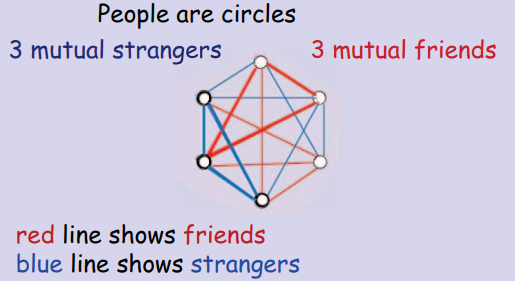
\includegraphics[width=0.8\textwidth]{../img/friends_and_strangers}
  \end{center}

  \begin{itemize}
  \item Six people, every two are either \alert{friends} or \structure{strangers}.
  \item {\bf Claim:} There is always a set of \alert{3 mutual
    friends} or \structure{3 mutual strangers}.
  \end{itemize}
  
\end{frame}

\begin{frame}
  \frametitle{Friends and Strangers, and Ramsey's Theorem}

  For any $k$, every \structure{large enough group} of people
  will contain $k$ mutual friends OR $k$ mutual strangers.
  
  \bigskip
  
  \begin{itemize}
  \item $R(3) = 6$
  \item $R(4) = 18$
  \item $R(5) = \text{ unknown!}$
  \end{itemize}
\end{frame}

\begin{frame}
  \frametitle{A bogus proof by cases: Prove $2a^2 > a$}
  \begin{enumerate}
  \item This proof is by case analysis.
  \item There are two cases:
    \begin{itemize}
      \item Case 1: $a$ is positive
      \item Case 2: $a$ is negative
    \end{itemize}
  \item One of these cases must always hold, because an integer is either positive or negative.
  \item Case 1: Suppose $a$ is positive.
  \item Since $a$ is an integer, we must have that $a \geq 1$.
  \item Hence, $2a^2 = 2a\times a \geq 2a\times 1 > a$.
  \item This implies the claim holds in Case 1.
  \item Case 2: Suppose $a$ is negative.
  \item Since $a$ is an integer, we must have that $a \leq -1$.
  \item Hence, $2a^2 \geq 2\times (-1 \times -1) = 2 > -1 \geq a$.
  \item This implies the claim holds in Case 2.
  \item The claim therefore holds in both cases. 
  \end{enumerate}
\end{frame}

\section{1.3 -- Weel Ordering Principle}
\subsection{Well Ordering Outline}

\begin{frame}
  \frametitle{The Well Ordering Principle}

  \begin{itemize}
  \item It is a very obvious (but very useful) principle in Mathematics;
    \bigskip
    
  \item It is so obvious that you have already used it without knowing;
  \end{itemize}
  
\end{frame}

\begin{frame}
  \frametitle{The Well Ordering Principle}

  {\Large
  \begin{center}
    Every non-empty set of\\
    \structure{Non-negative Integer Numbers}\\
    has one \alert{smallest element}
  \end{center}}
\end{frame}

\begin{frame}
  \frametitle{The Well Ordering Principle}
  \begin{center}
    Obvious? \structure{yes} \hspace{2cm} Trivial? \alert{no}
  \end{center}
  \vfill

  \begin{itemize}
  \item Every non-empty set of non-negative \structure{rational}
    numbers has one smallest element?

    \bigskip

  \item Every non-empty set of \structure{integers} numbers has one
    smallest element?
  \end{itemize}
\end{frame}

\begin{frame}
  \frametitle{Well Ordering Examples}
  {\large
    \begin{itemize}
    \item What is the smallest age of the U.Tsukuba students?
    \item What is the smallest number of cells in any animal?
    \item What is the smallest number of coins = 876 yens?
    \end{itemize}
  }
\end{frame}

\subsection{Sample Proof}
\begin{frame}
  \frametitle{Proof $\sqrt{2}$ is irrational using well ordering}

  \begin{itemize}
    \item if $\sqrt{2}$ is rational, then exist $m,n$ so that
      $\sqrt{2} = \frac{m}{n}$
    \item We can always find $m,n > 0$ such as they have no common
      factors.
    \item \alert{Why} always?
  \end{itemize}
\end{frame}

\begin{frame}
  \frametitle{Proof $\sqrt{2}$ is irrational using well ordering}
  \begin{itemize}
  \item Suppose that we choose the \alert{smallest} $m,n$.
    \bigskip
    
  \item Using the same idea as the previous proof, we show that both
    numbers must be divisible by two. ($m' = m/2, n' = n/2$)
    \bigskip
    
  \item Now we found a number \alert{smaller than the smallest! (contradiction!)}
  \end{itemize}
\end{frame}

\subsection{More Well Ordering Proofs}
\begin{frame}
  \frametitle{More Proofs Using the Well Ordering Principle}

  \begin{itemize}
  \item (Easy) Every integer $i > 1$ is a product of primes.

    \bigskip
    
  \item (Medium) Every number is \structure{Postal}.
    \begin{itemize}
    \item A number $n$ is postal if $n+8$ can be composed of a sum of
      ``threes'' and ``fives''
    \end{itemize}

    \bigskip

  \item (Difficult) $1 + r + r^2 + \ldots + r^n = \frac{r^n-1}{r-1}$
  \end{itemize}
\end{frame}

\begin{frame}
  \frametitle{General form for a Well Ordering proof}
  You want to prove that $\forall n \in \mathbb{N}, P(n)$ using WOP.
  
  \begin{enumerate}
  \item Define a set of counter examples $C$, $C ::=\{n \in
    \mathbb{N}|\text{ not } P(n)\}$
  \item Assume the minimum element of $C$ exists, $m$, by WOP
  \item Find a contradiction, for example:
    \begin{itemize}
    \item Find a contradiction $c \in C, c < m$;
    \item Show that $P(m)$ is actually True;
    \end{itemize}
    
  \end{enumerate}
\end{frame}

%\begin{frame}
%  \frametitle{Bogus WOP proof: Every Fibonacci Number is even}
%\end{frame}

\section{1.4 -- Propositions and Logic}

\begin{frame}
  \begin{center}
    Propositions and Logic
  \end{center}
\end{frame}

\subsection{Ambiguous Language}
\begin{frame}
  \frametitle{Why Mathematical Language?}

  \begin{itemize}
  \item Greeks carry swords or javelins.

    \bigskip

  \item Greeks carry bronze or copper swords.
  \end{itemize}
\end{frame}

\begin{frame}
  \frametitle{Mathematical Language}
  \begin{itemize}
  \item Mathematical Language helps create non-ambiguous statements.
    \bigskip
    
  \item We will not through all Logic operators here.
    \bigskip

  \item However, it is important to understand that they are based on
    \structure{binary} or \structure{boolean} logic.
  \end{itemize}
\end{frame}

%% Question -- Should I add slides on binary mathematical operations?
%% How do I segue into this topic?

\subsection{Truth Tables}
\begin{frame}
  \frametitle{Mathematical Language / Binary Logic}

  Example: X \structure{XOR} Y

  \bigskip

  \begin{tabular}{ll|l}
    X & Y & X XOR Y\\
    \hline
    TRUE & TRUE & FALSE\\
    TRUE & FALSE & TRUE\\
    FALSE & TRUE & TRUE\\
    FALSE & FALSE & FALSE\\
  \end{tabular}

  \bigskip

  \begin{itemize}
  \item A \structure{Truth Table} is a way to understand a logic
    operator.
  \item We can use logic operators to transform \alert{ambiguous natural
    language sentences} into \structure{clear logical propositions.}
    \begin{itemize}
    \item Greeks carry bronze or copper swords.
    \item Greek carry bronze sword XOR greek carry copper sword.
    \end{itemize}
  \end{itemize}
\end{frame}

\begin{frame}
  \frametitle{Binary Logic and Truth Tables}

  The \structure{truth table} allows us to analyze a logical formula:

  \bigskip
  
  \begin{itemize}
  \item Is it always true? Is it always false?
  \item Is it equivalent to another logical formula?
  \end{itemize}

  To analyze a formula using the truth table, I need to analyse the
  value of each variable.
\end{frame}

\begin{frame}
  \frametitle{Evaluation of a Formula}

  Given the following variables:\\ P = \structure{True}, Q = \structure{True}, R = \alert{False}

  \vfill
  
  How do we \structure{evaluate} the following formula?
  \begin{center}
    NOT(NOT(P) OR Q) AND (R OR (P XOR Q))
  \end{center}
\end{frame}

\begin{frame}
  \frametitle{Comparison of Two Formulas}

  We can decide whether two logical formulas are
  \structure{equivalent} if the final column of their truth table is
  identical.

  \vfill

  For example, let's prove DeMorgan's Law:
  \begin{center}
    NOT(P OR Q) \structure{equiv to} NOT(P) AND NOT(Q)
  \end{center}
\end{frame}

\subsection{Satisfiability}

\begin{frame}
  \frametitle{Satisfiability and Validity}

  \begin{itemize}
  \item A logic formula is \structure{satisfiable} if it is true for
    \alert{at least one} assignment.
  \item A logic formula is \structure{valid} if it is true for
    \alert{all} assignments.
  \end{itemize}

  \vfill

  \begin{itemize}
  \item \structure{Satisfiable:} NOT(B)
  \item \structure{Not Satisfiable:} B AND NOT(B)
  \item \structure{Valid:} B OR NOT(B)
  \end{itemize}
\end{frame}

\begin{frame}
  \frametitle{Checking for Validity and Satisfiability}

  Checking if a logic formula is satisfiable or not is a
  \structure{very importan problem} in CS.

  \bigskip

  But how to do it?

  \bigskip

  \alert{Alert!} If you try to use a truth table, the size of the
  table grows with the number of variables:
  \begin{itemize}
  \item 1 variable - 2 lines
  \item 2 variables - 4 lines
  \item 10 variables - 1024 lines
  \item n variables - $2^n$ lines...
  \end{itemize}  
\end{frame}

\begin{frame}
  \frametitle{Checking for Validity and Satisfiability}
  \begin{itemize}
  \item Is there an efficient way to test for satisfiability? (SAT)
    \bigskip
    
  \item The Efficient SAT problem is equivalent to the P=NP problem
    \bigskip
    
  \item The validity problem is also related to the SAT problem.
  \end{itemize}
\end{frame}

\section{1.5 -- Quantifiers}
\begin{frame}
  \begin{center}
    Logic Quantifiers
  \end{center}

  \bigskip
  \begin{itemize}
  \item For all: $\forall$
  \item Exists: $\exists$
  \end{itemize}
\end{frame}

\subsection{Predicates and quantifiers}
\begin{frame}
  \frametitle{What is a Predicate?}

  A predicate is a proposition with variables in it:

  \begin{equation*}
    P(X,Y) ::= [X+2 = Y]
  \end{equation*}

  \vfill

  The truth value of a predicate depends on the values of the variables:
  \begin{itemize}
  \item $X = 1, Y = 3$, P(X,Y) is True
  \item $X = 2, Y = 2$, P(X,Y) is False
  \end{itemize}
\end{frame}

\begin{frame}
  \frametitle{Quantifiers}

  \begin{itemize}
  \item $\forall x$ -- For ALL X
    
    \bigskip
    
  \item $\exists y$ -- There exists SOME Y
  \end{itemize}

  \vfill

  $\forall x$ works like \structure{AND}. For example:
  \begin{equation*}
    \forall x, x \in \{1,2,3\}|P(X) \text{ \alert{equiv} } P(1) \text{ AND } P(2) \text{ AND } P(3)
  \end{equation*}

  \bigskip

  $\exists y$ works like \structure{OR}. For example:
  \begin{equation*}
    \forall x, x \in \{1,2,3\}|P(X) \text{ \alert{equiv} } P(1) \text{ OR } P(2) \text{ OR } P(3)
  \end{equation*}
\end{frame}

\begin{frame}
  \frametitle{Quantifiers Example}

  For $x,y \in \mathbb{N}$ (x and y range over the integers).

  \begin{equation*}
    Q(Y) ::= \exists x. x < y.
  \end{equation*}

  \begin{itemize}
  \item Q(3) is \structure{True}. ($[x < 3]$ is T for $x = 1$)
  \item Q(1) is \structure{True}. ($[x < 1]$ is T for $x = 0$)
  \item Q(0) is \alert{False}. ($[x < 0]$ is not T for any $x\in\mathbb{N}$)
  \end{itemize}

  \bigskip

  What about a simple example for $\forall$?
\end{frame}

\begin{frame}
  \frametitle{Ordering Quantifiers}
  What is the difference when we order $\exists$ and $\forall$?

  \bigskip
  
  \begin{block}{Example 1: Medicines}
    $\forall d \in$ diseases. $\exists m \in$ medicine.\\
    $m$ cures $d$
  \end{block}

  \begin{block}{Example 2: Panacea}
    $\exists m \in$ medicine. $\forall d \in$ diseases.\\
    $m$ cures $d$
  \end{block}

  We need to be careful when writing mathematical notation!
  
\end{frame}

\begin{frame}
  \frametitle{Validity and Predicates}
  \begin{itemize}
  \item Propositional Validity: A \structure{proposition} is true for
    all truth assignments of variables.
    \begin{itemize}
    \item Example: (P implies Q) OR (Q implies P)
    \end{itemize}

    \bigskip
    
  \item Predicate Calculus Validity: A \structure{predicate} is valid
    when it is true for all domains.
    \begin{itemize}
    \item Example: $\forall z. [P(z) \land Q(z)] \rightarrow [\forall x.P(x) \land \forall y.Q(y)]$
    \end{itemize}
  \end{itemize}

  
\end{frame}

\section{Conclusion}
\begin{frame}
  \frametitle{Important Ideas from Lecture I}
  \begin{itemize}
  \item What are proofs?
  \item Proof techniques: Contradiction and Proof by Cases
  \item Proofs techniques can be used for debugging.
  \item What is the satisfiability problem.
  \item Why satisfiability is important to CS.
  \end{itemize}

  \bigskip
  
  Make sure to see video 1.5.4 from OCW!
  % TODO: Add material from video 1.5.4 here.
\end{frame}

\begin{frame}
  \frametitle{Exercise Sheet for Week 1}

  Please start working on the Exercise Sheet for Week 1. Deadline is
  Tuesday Next week (10/9).

  \vfill
  
  \begin{itemize}
  \item Each student must submit the exercise sheet separately.
  \item You may discuss the exercise with other students.
  \item You may ask the professor any questions.
  \item You may leave the classroom.
  \end{itemize}
  
\end{frame}

\end{document}
